\section{Introduction}

\begin{figure}
  \begin{center}
    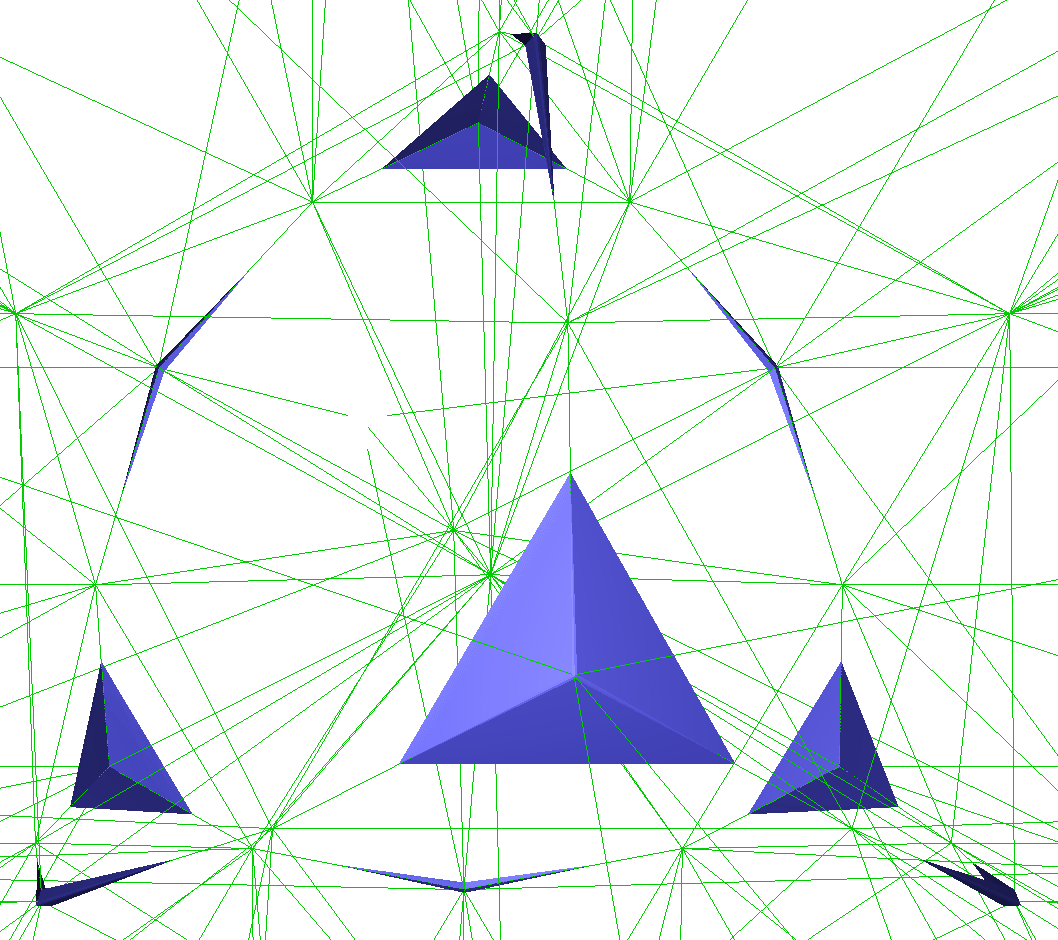
\includegraphics[width=\linewidth]{quartic-M-2.png}
    \caption{piecewise linear approximation of a quartic surface}
  \end{center}
\end{figure}

We present an algorithm solving smooth systems of homogeneous polynomial
equations $\{x ∈ \PNR, p₁(x) = 0, \dots, pₖ(x) = 0\}$. By \emph{smotth},
we mean than the vectors $(∇p₁(x),\dots,∇pₖ(x))$ are linearly independant for
all $x$. By
\emph{solving} we mean finding a piecewise linear approximation of the
solution that is homeomorphic to the real solution allowing for instance to
compute topological invariants of the solution and in particular the number of
connected components. We therefore do not limit ourselves to the zero
dimensional case.

To obtain the solution, we partition the projective space $\PNR$ is a
family of simplices $(Δⱼ)_{j∈J}$, then we construct
the piecewise linear functions $\overline{p}ᵢ$ that are linear on each $Δⱼ$ and
coincide with $pᵢ$ on the vertices of the simplices $Δⱼ$.

Then, we give a criteria to ensure that the set $\{x ∈ \PNR,
\overline{p}₁(x) = 0, \dots, \overline{p}ₖ(x) = 0\}$ is homeomorphic to the
solution of the original system.

The criteria can be summarised as follows:
\begin{itemize}
  \item For each point $x$ of $\PNR$, consider the set of simplices $\{Δ_{j₁},
    \dots, Δ_{jₘ}\} = \{Δⱼ, x ∈ Δⱼ\}$.
  \item For each polynomial $pᵢ$, this gives a set of $m+1$ vector: the gradient
    of the original polynomial $pᵢ$ at $x$, and the gradient of each linear
    function ${\overline{p}ᵢ}_{\restriction Δ_{jₖ}}$ at $x$:
    $$Gᵢ(x) = \{∇pᵢ(x),∇{\overline{p}ᵢ}_{\restriction Δ_{j₁}}(x),  \dots,
      ∇{\overline{p}ᵢ}_{\restriction Δ_{jₘ}}(x)\}$$
    \item Then the criteria is satisfied if for any $x \in \PNR$ such that ...
      and for any
      $(ε₁,\dots,εₖ) ∈ \{-,+\}ᵏ$, $0$ is not in the convex hull of
      $ε₁ G₁(x) ∪ \dots ∪ εₖ Gₖ(x) $.
\end{itemize}

This gives the spirit of the criterion. The real criterion needs a bit more care
as gradient of polynomials are not well defined
This criteria can be checked in practice with a sufficient condition as precise
as we want (up to more computation) using the fact that polynomials written in
the Berstein bases are in the convex hull of their coefficients.

The part of the algorithm is to construct a partition of $\PNR$ that satisfy the
above criterion. We are not yet able to prove that this part of our algorithm
terminates. But it does terminate in practice. It even seem that it requires a
partition whose size is bounded by a constant that only depends upon the number
of variables, number of polynomials and their degree (see conjecture \ref{?}).

Is important to remark that the correction of the algorithm only requires the
criterion to be proved correct, which is done in that paper.

%<!-- Local IspellDict: british -->
%<!-- Local IspellPersDict: ~/.ispell-british -->
